\section{Evaluation}
\label{sec:evaluation}

%% \begin{figure*}
%%     \centering
%%     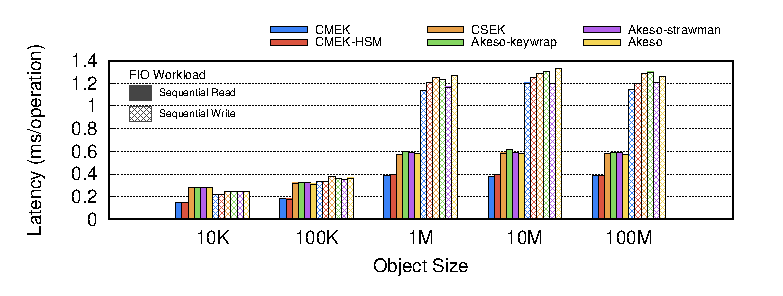
\includegraphics[width=\textwidth]{figs/fsop-latency-hist-2col}
%%     %
%%     \caption{Latency of read and write operations for encrypted cloud storage.}
%%     %
%%     \label{fig:fsop-latency-hist-2col}
%% \end{figure*}

To evaluate the performance of \SystemName, we wrote a series of micro-benchmarks in the library.
These microbenchmarks test each of the five main \SystemName PRE-related functions.
The results from running these benchmarks on an M1 Mac are shown below.

{\footnotesize
\begin{verbatim}goos: darwin
goarch: arm64
pkg: github.com/etclab/samba
cpu: Apple M1
BenchmarkEncrypt-8              	     358	   3157878 ns/op
BenchmarkDecrypt1-8             	     664	   1799279 ns/op
BenchmarkGenReEncryptionKey-8   	    1558	    770583 ns/op
BenchmarkReEncrypt-8            	     964	   1247834 ns/op
BenchmarkDecrypt2-8             	    1141	   1029601 ns/op
PASS
ok  	github.com/etclab/samba	6.129s
\end{verbatim}
}

The encryption performed by the external sender is the least expensive, which is good for responsiveness, since the user's request will be on its way relatively fast.
The generation of a re-encryption key and the use to that key to re-encrypt are more expensive.
Interestingly, the decryption of a re-encrypted message takes about twice as long as the decryption of a message encrypted under the original RSA.

To compare \SystemName's efficiency relative to cryptographic alternatives, we wrote functions and microbenchmarks for simple RSA, where we assume that either only one replica can exist for each function, or the proxy is trusted, and uses the leader's private key to decrypt and re-encrypt messages to the various replicas.
The benchmark results for RSA are shown below.

\color{red}
show RSA results

Compare the two

Show some figures

Justify the increased overhead
\color{black}


%
%% We will assess \SystemName's performance by measuring its overhead on
%% open-source AWS Lambda serverless applications, such as
%% CodePipeline\footnote{\url{https://github.com/aws-samples/aws-codepipeline-stepfunctions}}
%% and
%% MapReduce\footnote{\url{https://github.com/awslabs/lambda-refarch-mapreduce}},
%% which differ in chain length and complexity.
%% %
%% To decompose the overheads, we will compare \SystemName with: \emph{(1)}
%% \SystemName-strawman, which provides each function replica with the same key
%% pair via an enclaved key service; \emph{(2)} \SystemName-untrusted, which runs
%% functions in a non-confidential Oak VM; and \emph{(3)} standard OpenFaaS, using
%% OpenFaaS's default function runtime.
%% %
%% We will utilize the \texttt{wrk}\footnote{\url{https://github.com/wg/wrk}} and
%% Grafana \texttt{k6}\footnote{\url{https://grafana.com/oss/k6/}} benchmarking
%% tools to measure end-to-end latency, cold start times, and scalability.



%% \textbf{adwait}
%% 
%% % Evaluation (don't forget to interpret your data)
%% As no evaluation has taken place yet, I will lay out the steps by which we will likely evaluate the completed system. 
%% 
%% We will evaluate both the performance and cost of SAMBA, by answering the following research questions:
%% 
%% \newrq{rq:confidentiality}{How well does Samba ensure data confidentiality across functions without relying on centralized key management?}
%% 
%% \newrq{rq:control_flow_integrity}{How does Samba guarantee control flow integrity across function chains without a global controller?}
%% 
%% \newrq{rq:performance}{What is the performance overhead introduced by Samba's cryptographic protocols (proxy re-encryption and aggregate signatures) compared to unsecured FaaS usage, and comparable secure solutions?}
%% 
%% \newrq{rq:scalability}{How do Samba's decentralized key management system and aggregate signatures scale with large function graphs?}
%% 
%% To answer these research questions, we will design and implement Samba as an extension of Project Oak's Restricted Kernel.
%% We will evaluate Samba's security claims using some simple custom function-chain applications, and several real-world AWS-based applications (e.g., HelloRetail, CodePipeline, MapReduce).
%% 
%% \rqref{rq:confidentiality}
%% will be evaluated by simulating adversarial attempts from cloud providers to access encrypted inputs/outputs by running Samba in a VM on a "malicious" operating system.
%% \rqref{rq:control_flow_integrity}
%% will be evaluated by inserting malicious functions into a Samba chain and verifying whether deviations from the expected flow are detected and handled.
%% \rqref{rq:performance} and \rqref{rq:scalability}
%% will be measured using load-testing tools like \texttt{wrk} and \texttt{Grafana k6}, measuring end-to-end latency, cold start times, and autoscaling effectiveness, and comparing different Samba implementations with standard FaaS implementations.
%% 
%% \subsection{Confidentiality Evaluation}
%% We hypothesize that Samba doesn't leak any information to a malicious operating system.
%% This addresses \rqref{rq:confidentiality}.
%% We will deploy a chain of custom functions in Samba that runs properly, with all hardware and software described earlier.
%% Then, we will make attempts through the OS to read data from one of the Samba functions.
%% This simulates the case of an adversarial cloud provider.
%% We expect that no data will leak from within Samba to the OS. Success is defined as: All attempts by the OS to read data from within Samba fail.
%% 
%% \subsection{Control Flow Integrity Evaluation}
%% We hypothesize that Samba can detect and prevent unauthorized modification of data between functions in a graph, and unauthorized reordering of functions.
%% This addresses \rqref{rq:control_flow_integrity}.
%% We will deploy a chain of custom functions in Samba that runs properly, with all hardware and software described earlier.
%% Then, we'll reroute the ouput and input of two adjacent functions, respectively, to a "malicious" function, running on a non-TEE-based linux VM.
%% This simulates a man-in-the-middle scenario, where in insecure chains an adversary could read or change data.
%% We expect that no unauthorized party can reorder functions or modify data. Success is defined as:
%% \begin{enumerate}
%%     \item The function recieving input from the malicious function detects the invalid signature, throws an error, and ends execution.
%%     \item The malicious function is unable to decrypt any of the input it recieves from the previous function.
%% \end{enumerate}
%% 
%% \subsection{Cost Evaluation}
%% We hypotesize that we can provide the security guarantees of Samba with minimal performance overhead compared to standard FaaS platforms.
%% This addresses \rqref{rq:performance} and \rqref{rq:scalability}.
%% We will deploy several open-source AWS Lambda- and AWS Step-based FaaS applications, like HelloRetail, CodePipeline, and MapReduce.
%% We'll compare the performance our full Samba implementation with
%% \begin{enumerate}
%% \item a Samba implementation without proxy re-encryption, simply using a key service to provide each function with the same key pair,
%% \item a Samba implementation run on an unconfidential VM (no TEE), and
%% \item a standard OpenFaaS VM, with a standard runtime.
%% \end{enumerate}
%% We'll use wrk and Grafana to compare the performance.
%% We'll measure end-to-end latency, cold start times, and autoscaling behavior for our different environments.
%% Success is defined as maintaining minimal performance overhead (perhaps 10\%) compared to standard FaaS environments.
